\section{Data Dashboards in Data Science}
A data dashboard is a tool that businesses use to track, analyse, and display data, usually to gain a better understanding of the overall health of the organization, a department, or even a specific process. Dashboards connect a variety of metrics, data sources, APIs, and services behind the scenes, assisting businesses in extracting relevant information from those sources and displaying it in user-friendly ways. Data dashboards, similar to a car's dashboard, organize and display important information at a glance to help you understand your company's most valuable data and find answers to critical questions. By linking dashboards to specific metrics or key performance indicators (KPIs), you gain valuable business intelligence as well as the ability to delve deeply into specific pieces of information to continuously monitor success. Dashboards, like those in cars, show how far you are along your journey and how long it may take to get to your destination.
A dashboard's ability to provide up-to-date information and context to help inform business decisions and empower employees is one of its most powerful features. A dashboard, for example, could be used by an IT team to help detect signs of a security breach. Alternatively, a company could incorporate the dashboard into an app or mobile device for first-line workers in the field, ensuring that they have access to the data they require at all times.
As for the digital twin case in this paper, our paper will be used visualize data, forecast data for Nth number of years, make predictions on a given date, find out the impacts of parameters in your dataset and find out how to optimize the production line or produce the best outcome for your plant/company.
Our parameters (dataset headers example .csv) can be described as a set of

\begin{center}
    $\{p_n | n=p_1,p_2,p_2,\dots\}$
\end{center}

where $p_n$ is a parameter.\\


Let’s say for example in a water plant our $p_1$ can be DateAndTime , $p_2$ = PropertyMeasurement , $p_3$ = SomeChemicalCompound … $p_n$ = our dataset parameters for a given index
We could sketch graphs on this data and predict values based on parameter behaviors. We can play around, modify some parameters and see what effect that makes on our plant. Our AI can also optimize the plant for the best-fine-tuned results for our plant. It can generate insights for us and tell us how we can improve the quality of our plant or object. Below are examples of the dashboard and the functionality it presents to us.

\begin{figure}
    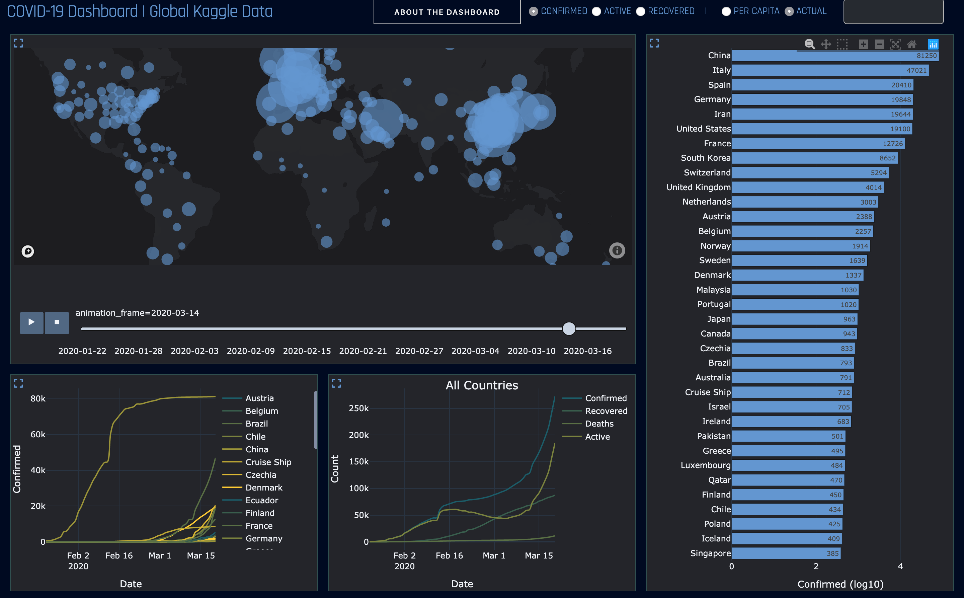
\includegraphics[width=\linewidth]{images/covid19dashboard.png}
    \caption{Example of a Covid-19 Dashboard just visualizing data with filters.}
    \label{fig:covid19dashboard}
\end{figure}

\begin{figure}
    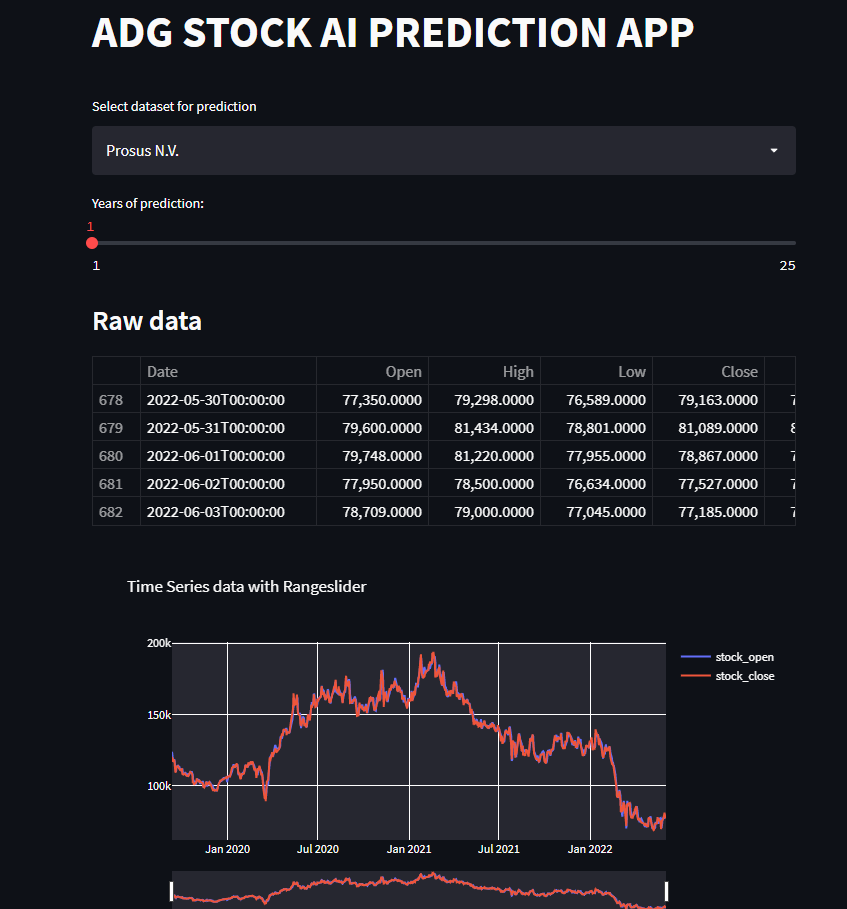
\includegraphics[width=\linewidth]{images/stonkapppt1.png}
    \caption{Example of my application dashboard displaying JSE stocks for a given date interval and forecasting stocks for a given number of years https://stonks.adgstudios.co.za}
    \label{fig:stonkapppt1}
\end{figure}

\section{Machine Learning and Forecasting}
\subsection{Introduction to Machine Learning and Forecasting for building digital twins}

Machine learning and forecasting are important tools in the digital twin toolbox. It is the most important component of the digital twin; without these tools and knowledge, the digital twin would not exist. Artificial Intelligence includes the subcategory of Machine Learning. Machine Learning is used to find trends/equations created from Machine Learning models that best describe our data and will be used to make predictions based on input and output data.
Let me describe the above in simple mathematical equations. \\

Let’s take our old-school way of a simple function/formula to determine some sort of output. Let us say
\begin{equation}
    \{p_n | n=p_1,p_2,p_2,\dots\}
\end{equation}

where $p_n$ is our parameters.\\

\textbf{General Equations we are taught in life} \\


\begin{equation}
    f(p_n)= p_n+rules
\end{equation}

\begin{equation}
    f(\{p_n | n=p_1,p_2,p_2,…\}) = \{p_n | n=p_1,p_2,p_2,…\}+rules \\
\end{equation}


\begin{center}
In Layman’s Equation Terms \\ 
Input + rules = output \\ 
\end{center}

\begin{center}
    (Input is put through the rules returning some form of output)
\end{center}


\textbf{In normal programming} \\

\begin{equation}
    \{p_n | n=p_1,p_2,p_2,…\}  +rules= ? 
\end{equation}

\begin{center}
    In Layman’s Equation Terms \\ 
    Input + rules = output \\ 
\end{center}

\begin{center}
    Our question mark represents (output, but depends on input and/or rules)
\end{center}

\textbf{In Machine Learning} \\ 

Let us define some machine learning equation let’s say if we are using the KNN algorithm (more about that later in this paper)

\begin{equation}
f(p_n )= f_{KNN} (p_n) \\
\end{equation}

\begin{equation}
f(\{p_n | n=p_1,p_2,p_2,…\})= f_{KNN} (\{p_n | n=p_1,p_2,p_2,…\}) \\ 
\end{equation}

\begin{center}
In Layman’s Equation Terms \\ 
Input + ? = output \\
\end{center}


\begin{center}
In this case the ? means the rules (program makes rules based on input and
expected output)
\end{center}
 
I have built a Python Module to find the best parameters to trains your machine learning module.
It is called adgmlclass which is on PyPi and code is open source on my GitHub.
You could also set the rules to a generic machine learning algorithm, modify the algorithm with fine-tuned Machine Learning parameters. 

\begin{figure}[H]
    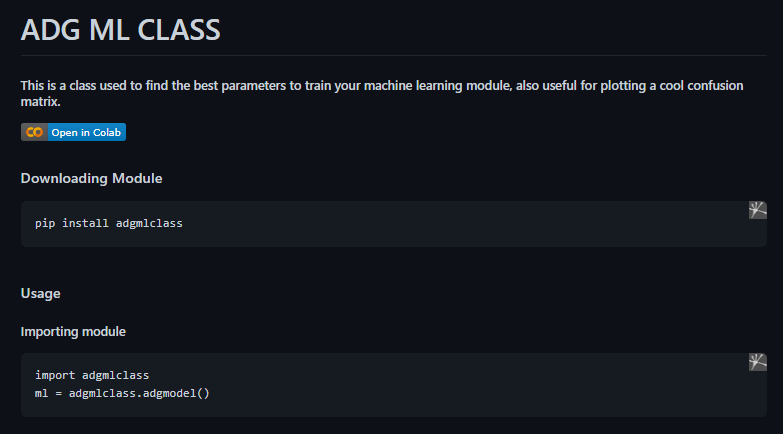
\includegraphics[width=\linewidth]{images/adgmlclassrepo.png}
    \caption{ADGMLCLASS : https://github.com/adgsenpai/adgmlclass}
    \label{fig:adgmlclass}
\end{figure}

\subsection{What is Machine Learning?}
Machine learning, also known as automatic learning, is a branch of science and a subcategory of artificial intelligence. It entails allowing algorithms to find "patterns" in data sets, i.e., recurring patterns. This information can take the form of numbers, words, images, statistics, and so on. Machine Learning can use anything that can be stored digitally as data.
Algorithms learn and improve their performance in performing a specific task by detecting patterns in this data.

\subsection{Which Mathematical Concepts Are Used in Machine Learning and Data Science?}
Statistics, Linear Algebra, Probability, and Calculus are the four key concepts that drive machine learning. While statistical concepts are at the heart of all models, calculus aids in the learning and optimization of those models.

\subsection{Importance of Machine Learning}
Machine learning is important because it allows businesses to see trends/predictions in customer behavior and business operational patterns while also assisting in the development of new products. Machine learning is at the heart of many of today's most successful businesses, including Facebook, Google, and Uber. In this paper, the importance of Machine Learning is that we are using it to predict and forecast data based on our input data which is the parameters to determine an output value on an output parameter.

\subsection{Machine Learning Types, Algorithms, and Usage}
\subsubsection{Types of Machine Learning:}
\textbf{Supervised Learning} \\ 
Supervised learning is a type of machine learning in which machine learning
from known datasets (set of training examples), and then predict the output.
A supervised learning agent needs to find out the function that matches a given sample set.
Supervised learning further can be classified into two categories of algorithms:
\begin{enumerate}
\item Classifications
\item Regression
\end{enumerate}

\textbf{Unsupervised Learning} \\ 
Unsupervised learning is associated with learning without supervision or 
training. In unsupervised learning, the algorithms are trained with data
which is neither labeled nor classified. In unsupervised learning,
the agent needs to learn from patterns without corresponding output values.
Unsupervised learning can be classified into two categories of algorithms:

\begin{enumerate}
\item Clustering
\item Association
\end{enumerate}


\textbf{Reinforcement Learning} \\ 
Reinforcement learning is a type of learning in which an AI agent is trained by giving some commands, and on each action, an agent gets a reward as feedback. Using these feedbacks, agent improves its performance. Reward feedback can be positive or negative which means on each good action, agent receives a positive reward while for wrong action, it gets a negative reward.
Reinforcement learning is of two types:
\begin{enumerate}
\item Positive Reinforcement learning
\item Negative Reinforcement learning
\end{enumerate}


\subsubsection{List of Common Machine Learning Algorithms}
% generate list
\begin{itemize}
\item \textbf{Linear Regression – (will explain the algorithm in paper)}
\item Logistic Regression
\item Decision Tree
\item SVM
\item Naive Bayes
\item \textbf{KNN – (will explain the algorithm in paper)}
\item K-Means
\item Random Forest
\item Dimensionality Reduction Algorithms
\item Gradient Boosting algorithms
\item Autoencoder
\item Convolutional Neural Network
\item Recurrent Neural Network
\item Support Vector Machine
\item Deep Learning
\end{itemize}

Deep learning is another complicated topic that I won't go into much detail about in this paper; instead, I'll give you some general information about it. Deep learning is a subset of a larger family of machine learning techniques based on representation learning and artificial neural networks. There are three types of learning: supervised, semi-supervised, and unsupervised. For image classification, object detection, image restoration, and image segmentation, deep learning has delivered superhuman accuracy—even handwritten digits can be recognized. Deep learning, which makes use of massive neural networks, is teaching machines to automate the tasks that human visual systems perform. Deep learning is a machine learning and artificial intelligence (AI) technique that mimics how humans acquire knowledge.

\begin{figure}[H]
    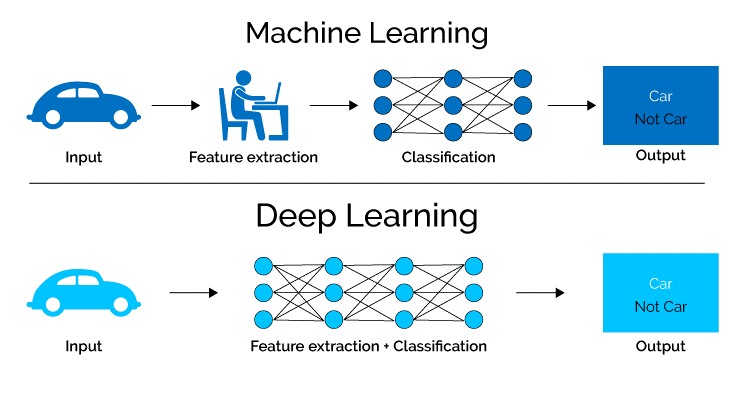
\includegraphics[width=\linewidth]{images/deeplearningdiagram.png}
    \caption{Deep Learning General Structure Diagram}
    \label{fig:deeplearningexplained}
\end{figure}

\subsection{Linear Regression}
\subsubsection{Introduction to Linear Regression}

A linear approach to modeling the relationship between a scalar response and one or more explanatory variables is known as linear regression in statistics. Simple linear regression is used when there is only one explanatory variable; multiple linear regression is used when there is more than one. 
Linear regression is a supervised machine-learning regression algorithm. \\
A typical linear regression equation that you learned in high school is in the form of
\begin{equation}
y = b_0 + b_1 x
\end{equation}

where $y$ is the response variable, $b_0$ is the intercept, and $b_1$ is the coefficient. \\

\begin{figure}[H]
    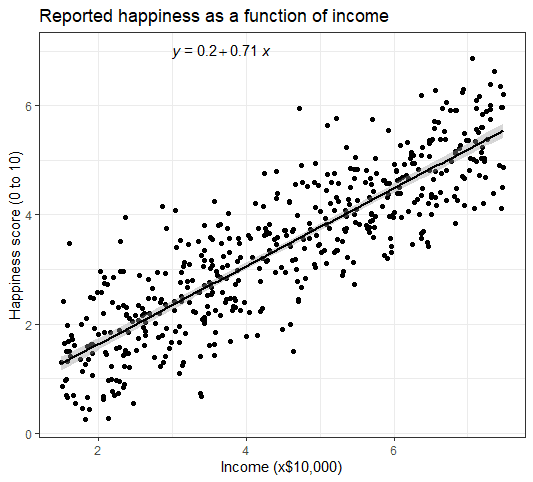
\includegraphics[width=\linewidth]{images/linearregeg.png}
    \caption{Linear Regression function of Reported Happiness by income values}
    \label{fig:linearregressionfunction}
\end{figure}

In this example, employees are interviewed and are asked to fill in the form below.
Rate your happiness in life from 

\begin{equation}
y \in \left\{0..10\right\} 
\end{equation}
 
We capture our data and represent it in a digital format or record it on a page.
The data scientist visualizes the data in a scatter graph. To make predictions on this data he calculates the regression equation which is 

\begin{equation}
y=0.2+0.71x 
\end{equation}

and plots the function on the scatter graph. If you look at the diagram above that is exactly what is being done to predict data. \\

\textbf{Simple Prediction and Flaw with Linear Regression} \\ 
Let us predict my happiness score based on this model. \\ 

where $x$ is the income in 10k \\
and $y$ is the happiness score.

\begin{equation}
    y=0.2+0.71(100)
\end{equation}

Our predicted score is \textbf{71.2}. That is not possible as the scale can only be $y \in \left\{0..10\right\}$
You can see that the model above is invalid and inaccurate. The training size is too small. We could get a better model if we use a larger population. The point I’m trying to make with Linear Regression is that you will get false alerts and reading based on the input data. I would also say emotions with people are not accounted for when working with Machine Learning models. For example, some people who are multi-millionaires are depressed with life. Some people with low income are happy in life they appreciate the simple things in life. Machine Learning does not account for emotion there is another aspect in AI that can help predict emotions and that is called Natural Language Processing. It works with text and speech. Deep learning powers that technology.\\

\textbf{Other types of Linear Regression} \\
What I showed you in the introduction was a \textbf{simple linear regression} equation which is 
\begin{equation}
y = b_0 + b_1 x
\end{equation}

where $y$ is the response variable, $b_0$ is the intercept, and $b_1$ is the coefficient. \\

A simple graph of that is 
\begin{figure}[H]
    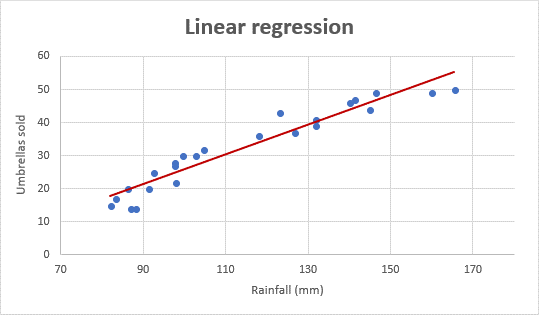
\includegraphics[width=\linewidth]{images/simplereg.png}
    \caption{Simple Linear Regression}
    \label{fig:simplelinearreg}
\end{figure}

The second type of linear regression is called \textbf{Multiple Linear Regression}
\begin{equation}
y = \beta_0 + \beta_1 x_1 + \beta_2 x_2^2 + \cdots + \beta_n x^n
\end{equation}
    
    where $y$ is the response variable, $\beta_0$ is the intercept, and $\beta_1$ is the coefficient for $x_1$, $\beta_2$ is the coefficient for $x_2^2$, and so on. \\


\begin{figure}[H]
    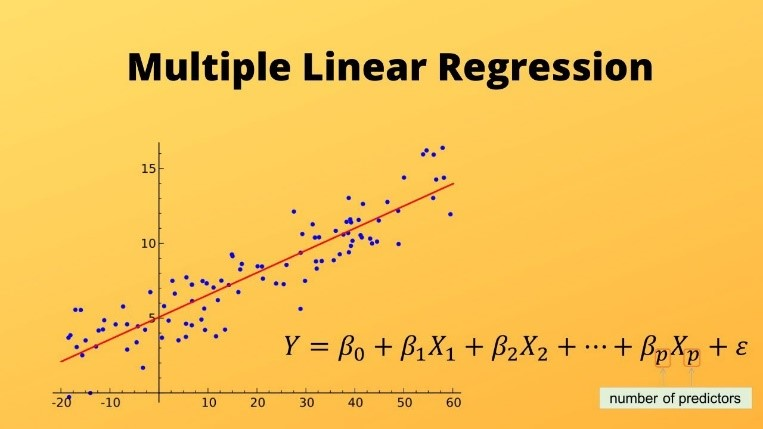
\includegraphics[width=\linewidth]{images/mlrgraph.jpg}
    \caption{Multiple Linear Regression}
    \label{fig:mlr}
\end{figure}


A graph for multiple linear regression looks similar to the simple linear regression above.

The last type of linear regression is called \textbf{Polynomial Linear Regression}
\begin{equation}
y = \beta_0 + \beta_1 x_1 + \beta_2 x_1^2 + \cdots + \beta_n x_1^n
\end{equation}
    
    where $y$ is the response variable, $\beta_0$ is the intercept, and $\beta_1$ is the coefficient for $x_1$, $\beta_2$ is the coefficient for $x_1^2$, and so on. \\
 
    \begin{figure}[H]
        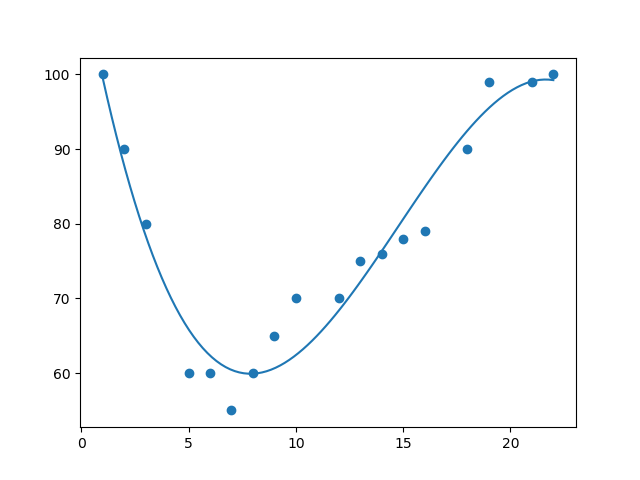
\includegraphics[width=\linewidth]{images/plr.png}
        \caption{Multiple Linear Regression}
        \label{fig:plr}
    \end{figure}
    
\subsection{K-Nearest Neighbors}
\subsubsection{Introduction to K-Nearest Neighbors}
K-nearest neighbors (k-NN) is a supervised machine learning algorithm that can be used to solve both classification and regression tasks.
Suppose there are two categories, i.e., Category A and Category B, and we have a new data point x1, so this data point will lie in which of these categories. To solve this type of problem, we need a K-NN algorithm. With the help of K-NN, we can easily identify the category or class of a particular dataset. \\ Consider the below diagram:

    \begin{figure}[H]
        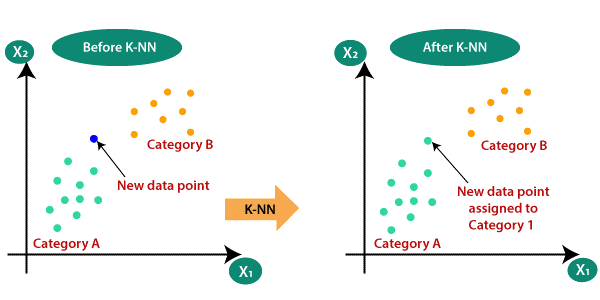
\includegraphics[width=\linewidth]{images/knnexp.png}
        \caption{K-Nearest Neighbors}
        \label{fig:knn}
    \end{figure}
    
    The K-NN algorithm is a supervised machine learning algorithm that can be used to solve both classification and regression tasks. \\

\textbf{How does the k-nearest neighbors algorithm work?} \\

\begin{enumerate}
\item Select the number K of the Neighbors
\item Calculate the Euclidean distance of K number of neighbors
\item Take the K nearest neighbors as per the calculated Euclidean distance.
\item Among these k neighbors, count the number of the data points in each category.
\item Assign the new data points to that category for which the number of the neighbour is maximum.
\end{enumerate}

Suppose we have a new data point and we need to put it in the required category.
\begin{figure}[H]
        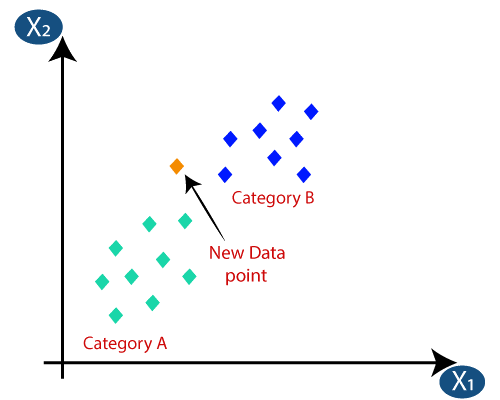
\includegraphics[width=\linewidth]{images/knnexp2.png}
        \caption{K-Nearest Neighbors Datapoint Graph}
        \label{fig:knndp}
\end{figure}
 
\begin{itemize}
\item Firstly, we will choose the number of neighbors, so we will choose the k=5.
\item Next, we will calculate the Euclidean distance (which we learnt in high school) between the data points. The Euclidean distance is the distance between two points, which we have already studied in geometry. It can be calculated as:
\end{itemize}
\begin{equation}
    {D_{Euclidean}} = \sqrt{(x_1-x_2)^2 + (y_1-y_2)^2}
\end{equation}

\begin{figure}[H]
    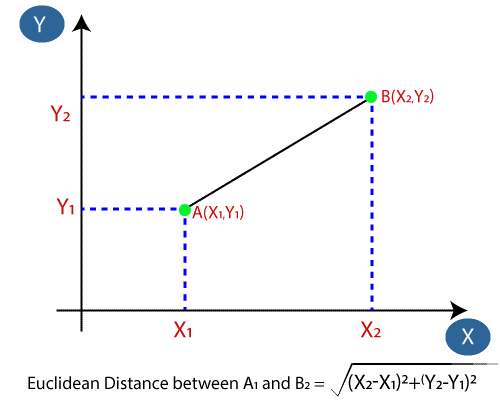
\includegraphics[width=\linewidth]{images/knnexp3.png}
    \caption{Calculating Euclidean distance between two data points}
    \label{fig:exp3}
\end{figure}

By calculating the Euclidean distance, we got the nearest neighbors, as three nearest neighbors in category A and two nearest neighbors in category B. Consider the below image:
\begin{figure}[H]
    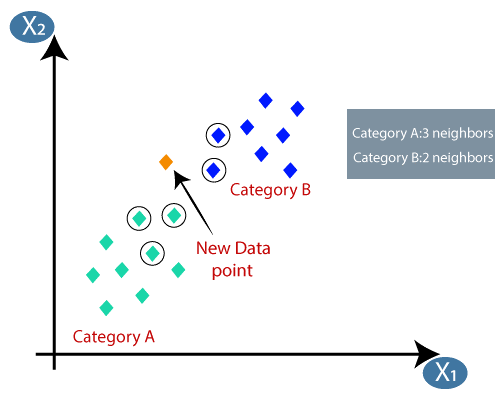
\includegraphics[width=\linewidth]{images/knnexp4.png}
    \caption{Nearest Neighbors}
    \label{fig:knnexp4}
\end{figure}

As we can see the 3 nearest neighbors are from category A, hence this new data point must belong to category A. \\

\textbf{Advantages of KNN Algorithm} \\
\begin{itemize}
\item It is simple to implement.
\item It is robust to the noisy training data
\item It can be more effective if the training data is large.
\end{itemize}

\textbf{Disadvantages of KNN Algorithm} \\
\begin{itemize}
\item Always needs to determine the value of K which may be complex some time.
\item The computation cost is high because of calculating the distance between the data points for all the training samples.
\end{itemize}

\textbf{Distance functions} \\ 

For KNN we can use different distance functions to achieve better accuracy or different K values.

% Euclidean Formula
\begin{equation}
    {D_{Euclidean}} = \sqrt{(x_1-x_2)^2 + (y_1-y_2)^2}
\end{equation}

%Manhattan  Formula
\begin{equation}
    {D_{Manhattan}} = |x_1-x_2| + |y_1-y_2|
\end{equation}

%Minkowski Formula
\begin{equation}
    {D_{Minkowski}} = \left\{ \left[ \left( \left( x_1-x_2 \right)^p \right)^q \right]^r \right\}^{1/r}
\end{equation}

\subsection{Measuring of Performance of Models}

We can use functions in our machine learning libraries to measure performance of our model.

    \begin{figure}[H]
        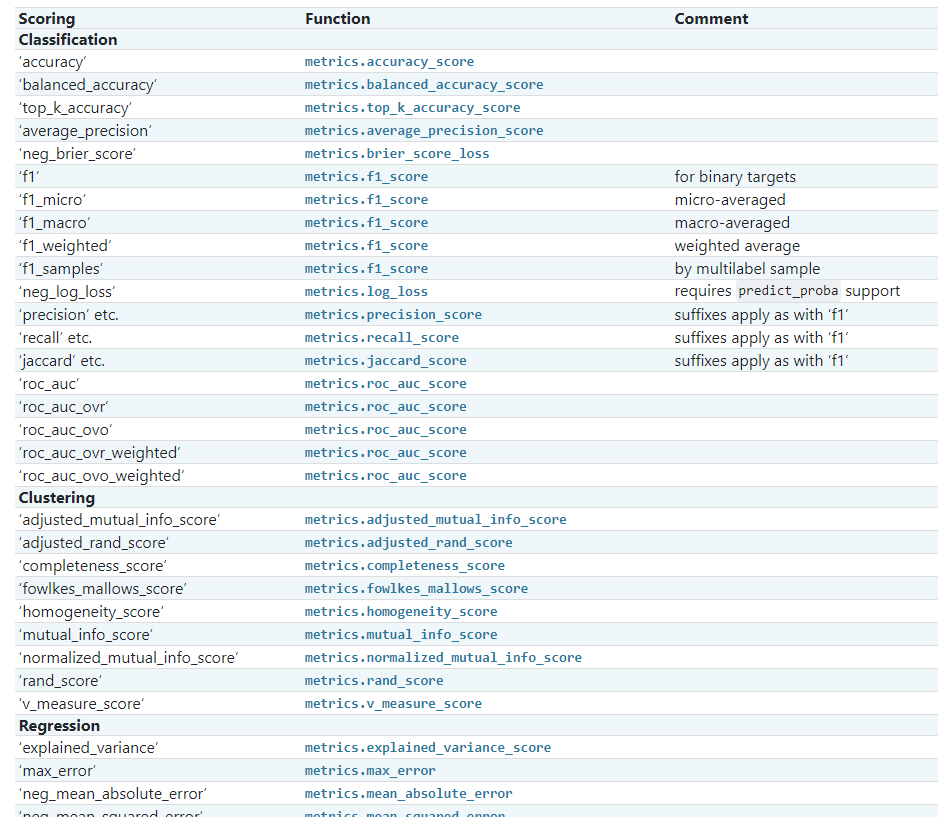
\includegraphics[width=\linewidth]{images/performance.png}
        \caption{Performance measurement functions in Python Scikit-Learn Module}
        \label{fig:perf}
    \end{figure}

above is a photo of performance metrics functions for the module scikit-learn in Python if you research these function names you can view formulas on these tools.

Check out the following link for more information on performance metrics:

\url{https://scikit-learn.org/stable/modules/model_evaluation.html}

\subsubsection{Real life example of model evaluation}

Below is performance metrics on a model I improved on a project of Galaxy Machine Learning.

\begin{figure}[H]
    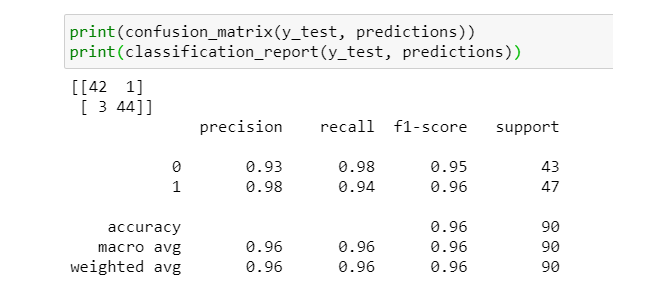
\includegraphics[width=\linewidth]{images/performancemetrics.png}
    \caption{Performance metrics on a model}
    \label{fig:perfex}
\end{figure}

For the model above you can see it has extremely good accuracy of around 96\% accuracy
Anything above 90\% I consider good enough there was times I even got 100\% accuracy for a model. \\
Let’s check out how our F1-Score is calculated. \\

\begin{equation}
    F1\textnormal{-}Score = \frac{2 \times Precision \times Recall}{Precision + Recall}
\end{equation}

alternatively, we can use the following formula:

    \begin{equation}
        F1\textnormal{-}Score = \frac{2TP}{2TP+FP+FN}
    \end{equation}

where TP is the number of true positives, FP is the number of false positives, FN is the number of false negatives. \\

\textbf{What does TP mean?} \\
That means True Positives in our dataset. Which our correct data in our dataset which tested true in our data. \\
\textbf{What does FP mean?} \\
That means False Positives in our dataset. Which our incorrect data in our dataset which tested false in our data. \\
\textbf{What does FN mean?} \\
That means False Negatives in our dataset. Which our incorrect data in our dataset which tested true in our data. \\






Another tool we can use to showcase our TP, FP, FN is called a \textbf{confusion matrix}

Mathematically, a confusion matrix looks like this:

\begin{equation}
    \begin{bmatrix}
        TP & FP \\
        FN & TN
    \end{bmatrix}
\end{equation} \\

Graphically could look like this below
\begin{figure}[H]
    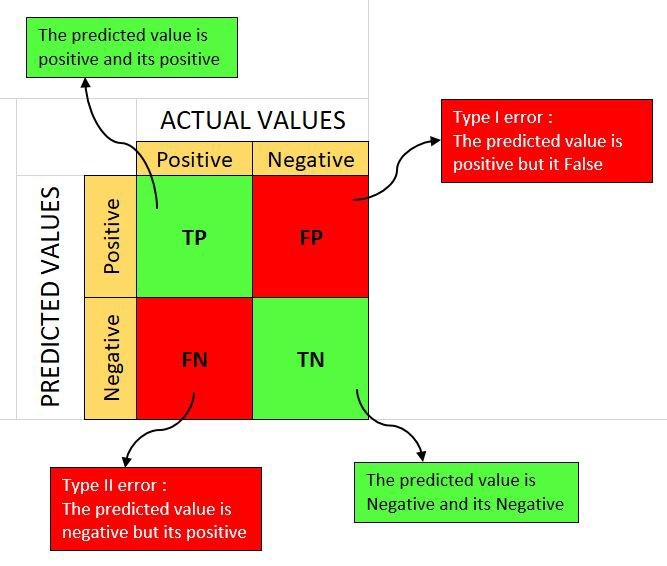
\includegraphics[width=\linewidth]{images/confusionmatrix.jpg}
    \caption{Confusion Matrix}
    \label{fig:confusion}
\end{figure}

Another graphical representation using the ADGMLCLASS library is shown below:
\begin{figure}[H]
    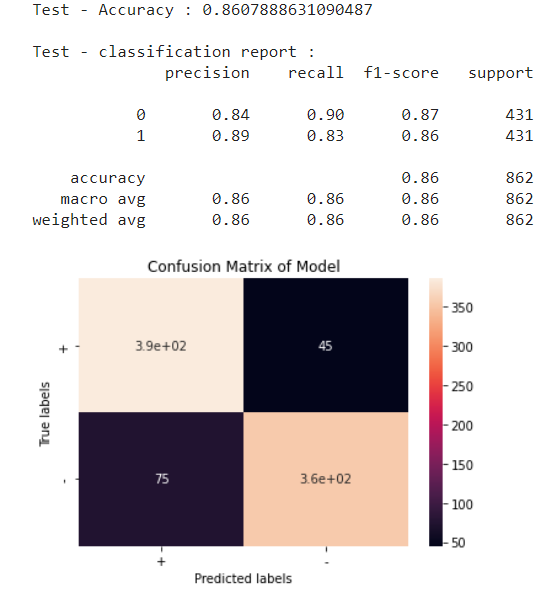
\includegraphics[width=\linewidth]{images/confusionmatrixpt2.png}
    \caption{Real life Confusion Matrix of a model}
    \label{fig:confusion2}
\end{figure}

\subsection{Playing with Machine Learning Demos + Real World Examples I did}

\subsubsection{GalaxyML}

You can play with GalaxyML. I helped a masters student optimize the ML Solution using adgmlclass and put the repo because this is a real-world example of ML in action.  

\begin{figure}[H]
    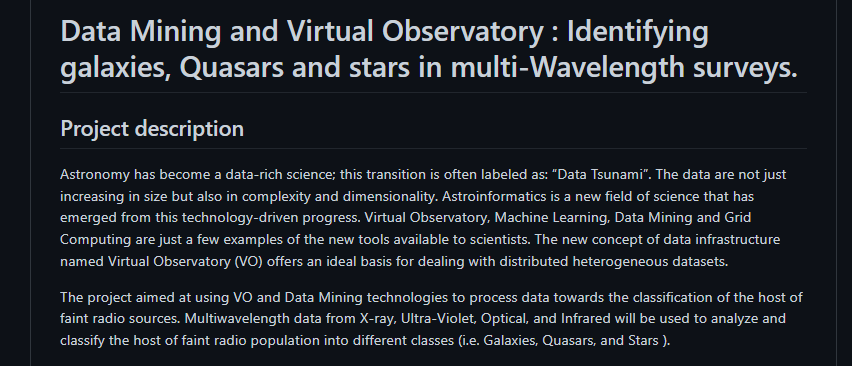
\includegraphics[width=\linewidth]{images/galaxymlrepo.png}
    \caption{GalaxyML Repo}
    \label{fig:galaxyml}
\end{figure}

\begin{center}
    \url{https://github.com/ADGSTUDIOS/GalaxyML}
\end{center}

\subsubsection{Neural Networks}
\begin{figure}[H]
    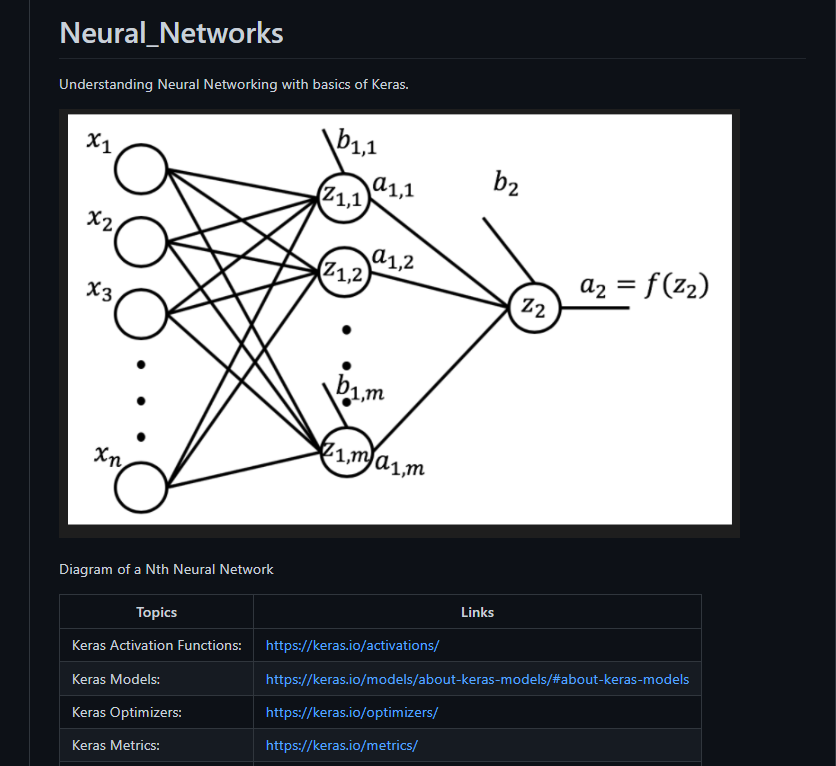
\includegraphics[width=\linewidth]{images/neuralnetworksrepo.png}
    \caption{Neural Networks Repo}
    \label{fig:neuralnetworks}
\end{figure}

If you want to play with Neural Networks got great notebooks to play with @ 
\url{https://github.com/adgsenpai/Neural_Networks}

\subsubsection{Machine Learning Application in ECommerce}

Clothing Size Guide AI Application used for predicting clothing size \\
given a users BUST(CM) and HIPS(CM) \\ 

\begin{figure}[H]
    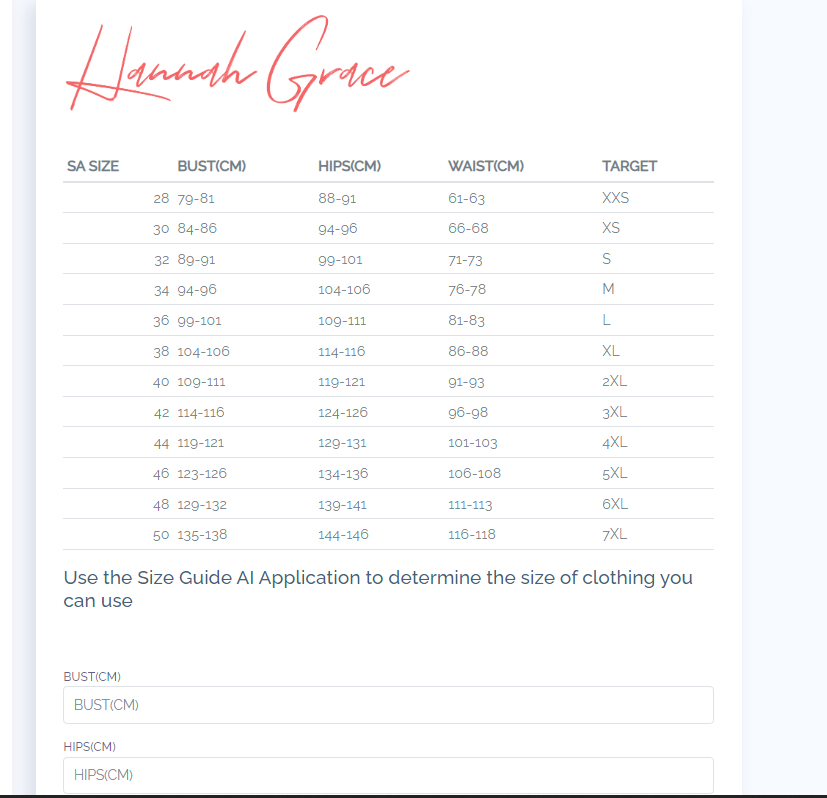
\includegraphics[width=\linewidth]{images/hannahgrace.png}
    \caption{Hannah Grace Clothing Size AI Application}
    \label{fig:clothingai}
\end{figure}

you can play with it @ \url{https://www.hannahgrace.co.za/size-guide/} this app has an accuracy of 100\%